\subsection{Display Comparison}
The main difference between vector and raster displays, is that vector displays draws the image by scanning primitives, and a raster display draws the image by using scanlines.

While a CRT raster display scans repeatedly in a fixed pattern, a vector display scans lines by gradually firing the electron beam to a point defined by two voltages: one defining the horizontal placement X and one defining the vertical Y.
Once a line is drawn, the electron emitter stops firing and moves to the starting point of the next line, thus leaving out dark areas.
This process is shown in figure \ref{fig:vectorscan}.

As vector displays are able to draw directly from one point to another, they do not suffer from artifacts such as aliasing and pixelation, which are present in raster displays ~\cite{vector-monitor}.
However, graphic complexity on vector displays are very limited compared to raster screens.

\begin{figure}[h!]
\centering 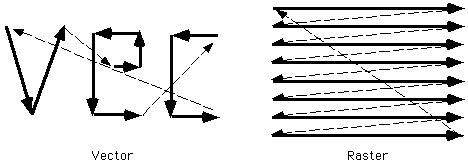
\includegraphics[width=0.8\linewidth]{images/scan.png}
\caption{Scan comparison between vector graphics and raster graphics ~\cite{vecvsras}.}
\label{fig:vectorscan}
\end{figure}

After an image has been drawn, both display types need to make the image stay put so that it can be perceived by humans.
Some CRT displays use phosphor types that fade out very quickly and needs redrawing 30-40 times per second ~\cite{vector-monitor}.
However, special types of phosphor can last for several minutes.
Modern raster displays have the advantage that once an image has been 'configured' in the display, the hardware makes it remain as long as the display is powered.
Thus, no constant redrawing is necessary ~\cite{LCD-persistence}.
Movies are nothing more than successive images drawn to the display.

Screen flickering is an artifact caused by lower refresh rates than the human eye perceives as natural motion, and can occur in both display types ~\cite{flicker}.
On vector displays, the entire screen does not have to be scanned every time, only the areas that the electron beam has to light up.
However, the sometimes irregular electron beam motion is often slower than raster screens' predictable scanning ~\cite{vecvsras}.
As a result, the refresh rate of a vector display is more easily prone to flickering, since it has no way of limiting the scene size.
When more primitives need to be drawn, the display will start to flicker more frequently.
A raster display guarantees that all pixels will be updated within a specified refresh rate, since the number of pixels always stays the same.
